
%%%%%%%%%%%%%%%%%%%%%%% file typeinst.tex %%%%%%%%%%%%%%%%%%%%%%%%%
%
% This is the LaTeX source for the instructions to authors using
% the LaTeX document class 'llncs.cls' for contributions to
% the Lecture Notes in Computer Sciences series.
% http://www.springer.com/lncs       Springer Heidelberg 2006/05/04
%
% It may be used as a template for your own input - copy it
% to a new file with a new name and use it as the basis
% for your article.
%
% NB: the document class 'llncs' has its own and detailed documentation, see
% ftp://ftp.springer.de/data/pubftp/pub/tex/latex/llncs/latex2e/llncsdoc.pdf
%
%%%%%%%%%%%%%%%%%%%%%%%%%%%%%%%%%%%%%%%%%%%%%%%%%%%%%%%%%%%%%%%%%%%


\documentclass[runningheads]{llncs}

\usepackage{amssymb}
\setcounter{tocdepth}{3}
\usepackage{graphicx}
\usepackage[latin1]{inputenc}
\usepackage{color}
%\usepackage{txfonts}

\usepackage{url}
\urldef{\mailsa}\path|R.Bordini@durham.ac.uk|
\urldef{\mailsb}\path|{hubner,picard}@emse.fr|
\newcommand{\keywords}[1]{\par\addvspace\baselineskip
\noindent\keywordname\enspace\ignorespaces#1}

\newcommand{\comment}[2]{\noindent\textsf{
    \begin{center}
      \colorbox[rgb]{.8,.8,.8}{
          \begin{minipage}{.95\columnwidth}
            {{#1 :}} \\ {#2}
          \end{minipage}
        }
    \end{center}
  }
}

\newcommand{\ascomment}[1]{\comment{\emph{AgentSpeak}}{#1}}

\begin{document}

\mainmatter  % start of an individual contribution

% first the title is needed
\title{Role Dynamics in the \emph{Jason} Team}
\subtitle{Agent Contest 2008}
% a short form should be given in case it is too long for the running head
\titlerunning{Jason Team's Role Dynamics}

% the name(s) of the author(s) follow(s) next
%
% NB: Chinese authors should write their first names(s) in front of
% their surnames. This ensures that the names appear correctly in
% the running heads and the author index.
%
\author{Rafael H. Bordini{$^\star$} \and Jomi F. H{\" u}bner{$^\dagger$} \and Gauthier Picard{$^\dagger$}}
%
\authorrunning{Bordini, H\"ubner and Picard}
% (feature abused for this document to repeat the title also on left hand pages)

% the affiliations are given next; don't give your e-mail address
% unless you accept that it will be published
\institute{
{$^\star$}~University of Durham, UK\\
\mailsa\\
{$^\dagger$}~\'Ecole des Mines de Saint-\'Etienne, France\\
\mailsb\\
% \mailsc\\
\url{http://jason.sourceforge.net/}}

%
% NB: a more complex sample for affiliations and the mapping to the
% corresponding authors can be found in the file "llncs.dem"
% (search for the string "\mainmatter" where a contribution starts).
% "llncs.dem" accompanies the document class "llncs.cls".
%

%\toctitle{Lecture Notes in Computer Science}
%\tocauthor{Authors' Instructions}
\maketitle


\begin{abstract}
This document presents the main ideas concerning the dynamics of the role within the \emph{Jason} team. An agent's life cycle is decomposed into two phases: \emph{exploration} and \emph{herding}. During each of these two phases, an agent will play different roles according to the context (cluster size, number of herders, etc.). 

\keywords{Jason, organisation, roles}
\end{abstract}


\section{Introduction}

As to remind the roles identified in the AC 2008 proposal we made, Figure \ref{fig:groups} presenting the group structure in the \emph{Jason} team.

\begin{figure}[h]
  \centering
  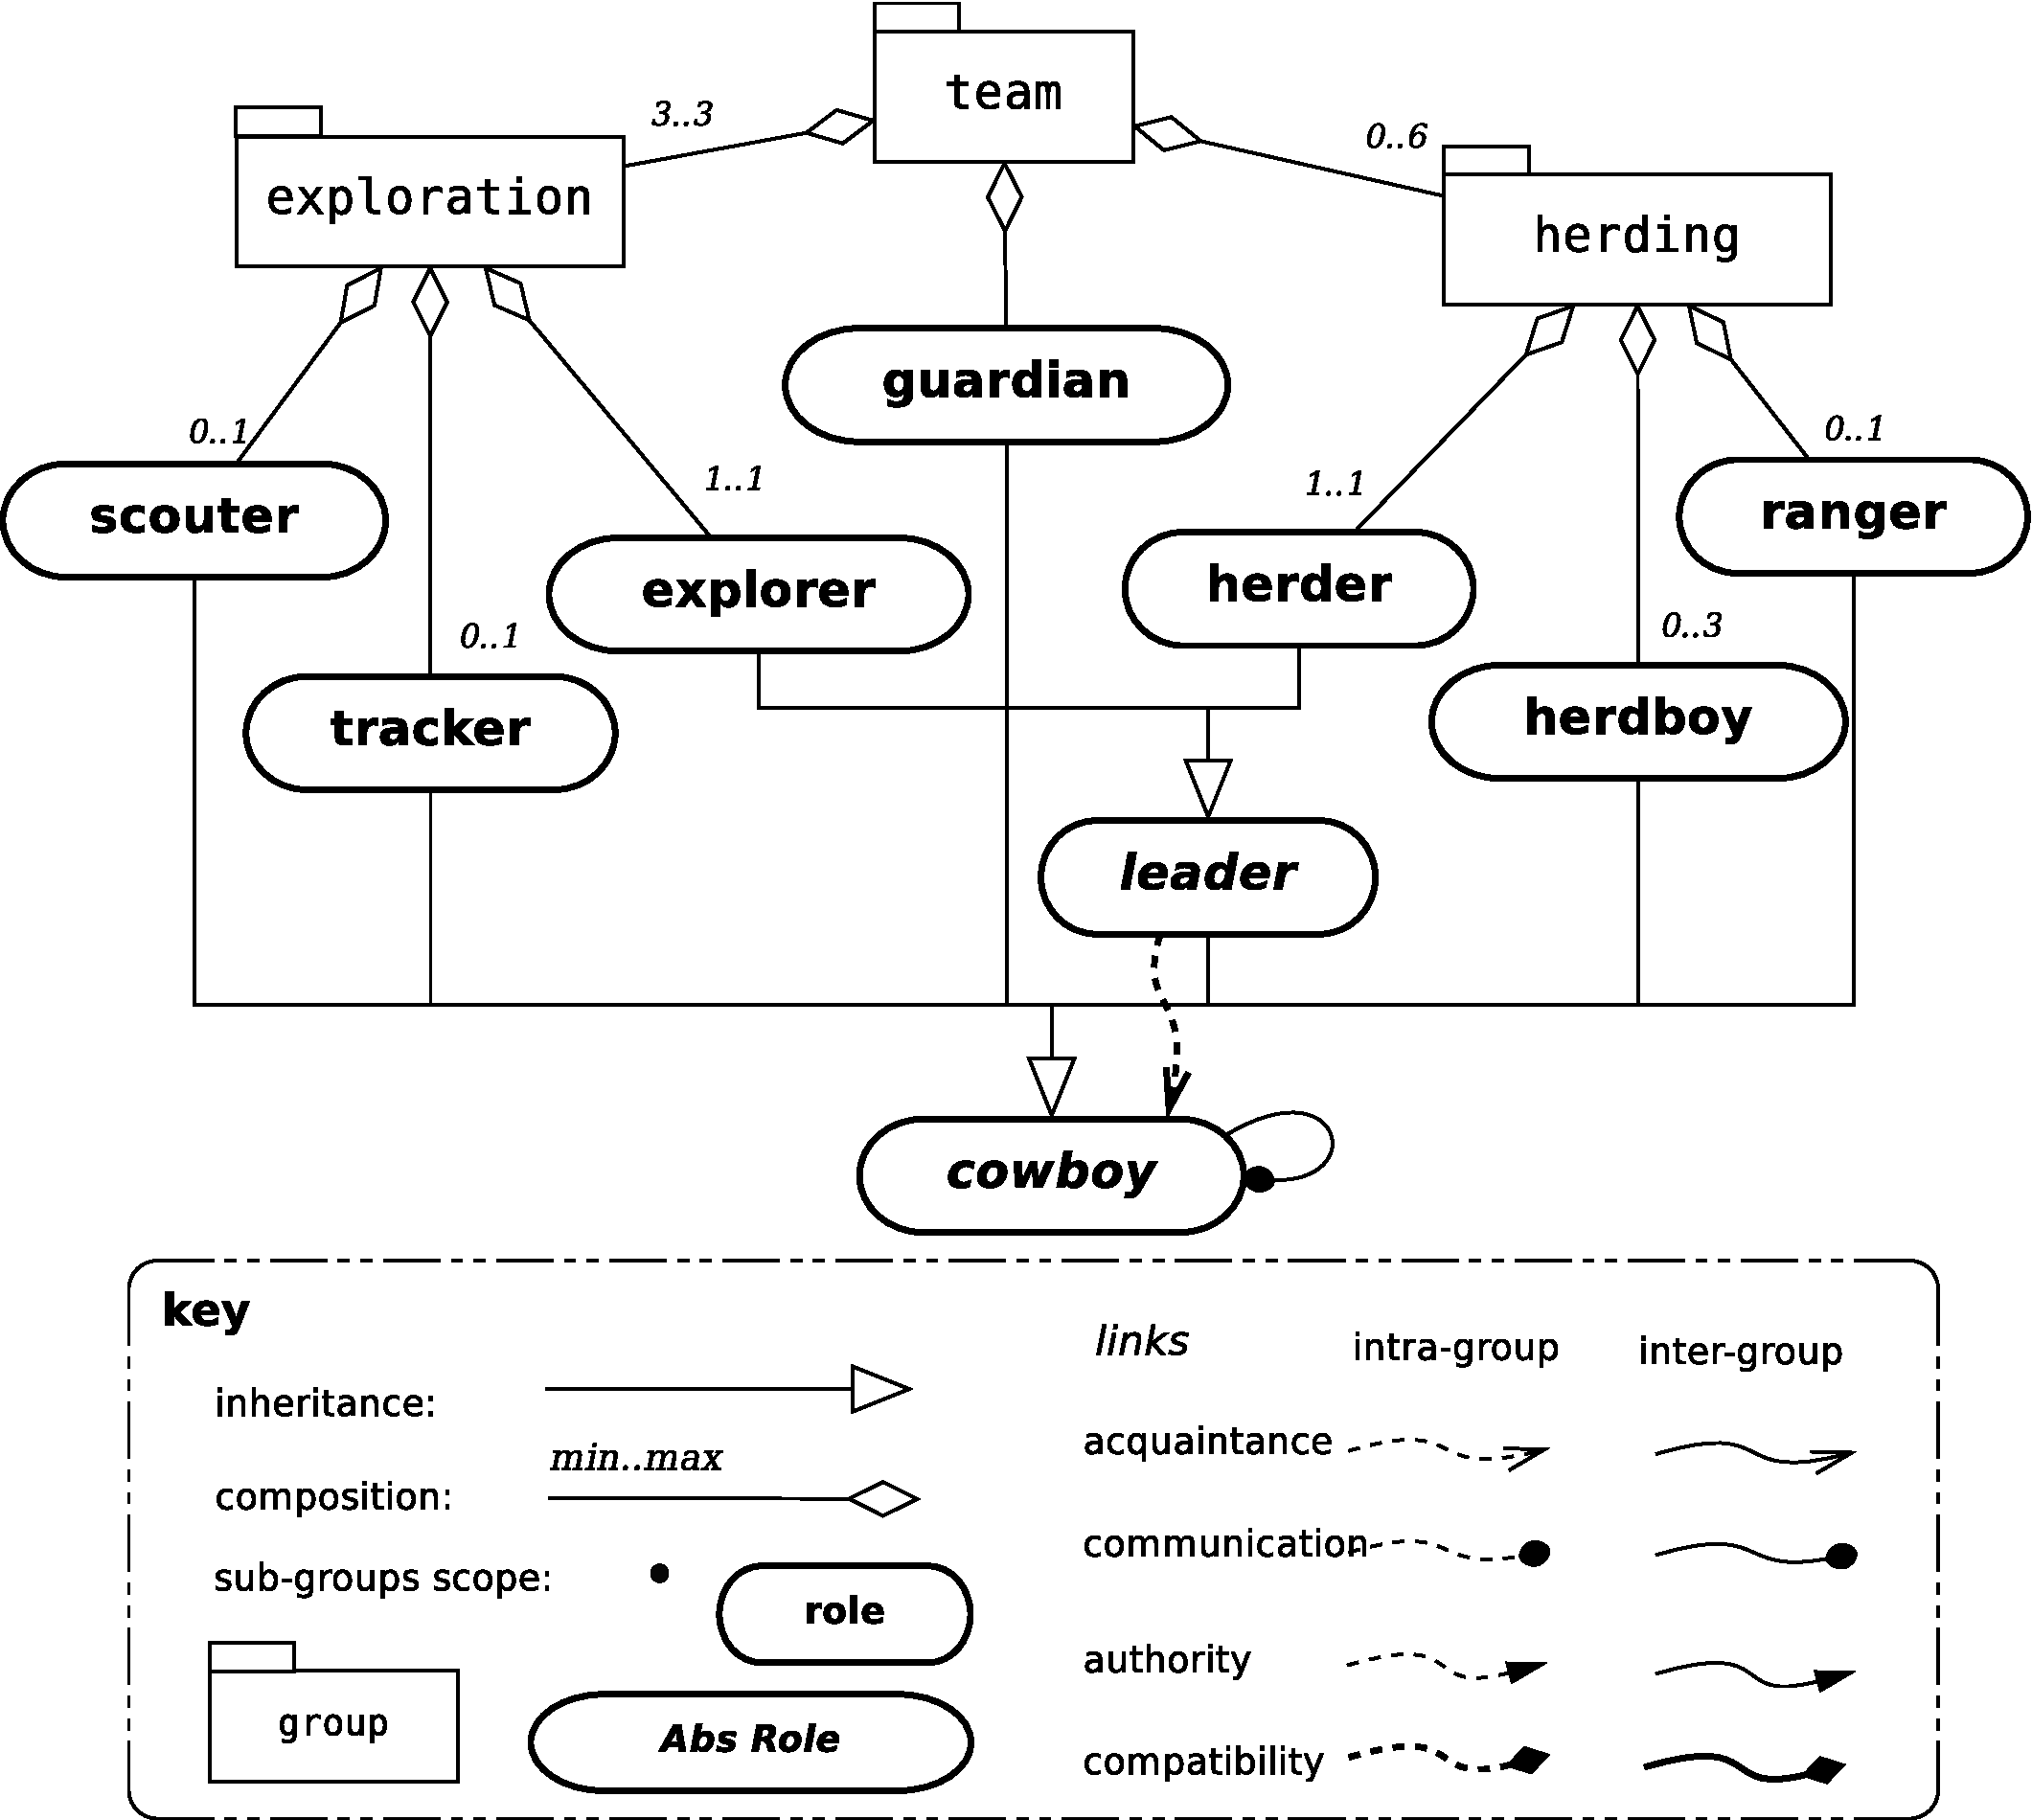
\includegraphics[width=0.8\columnwidth]{figures/jason-team-SS.pdf}
  \caption{Role and group structures}
  \label{fig:groups}
\end{figure}

Here is a reminder of the specific roles:

\begin{itemize}
\item \textit{guard}: guards the corral so as to keep the herded cows
  safe inside it;
% exploration group roles
\item \textit{explorer}: explore the environment until it detects a cow;
\item \textit{scout}: follows the explorer;
\item \textit{tracker}: once a cow is detected, tracks all cows of a cluster
  so as to evaluate its size;
  % \item \textit{perturbator}: perturbs the other team (only triggered if the
  %   other team is not fairplay),

% hersing group roles
\item \textit{herder}: herds the cows detected by explorer to reach
  the corral (since they move quicker than cows, they can also
  continue to explore around the cluster);
\item \textit{herdboy}: helps the herder to lead cows to the corral;
\item \textit{ranger}: finds the ``best'' path to the corral.
\end{itemize}

Actually, an agent will follow a simple life cycle: exploration, herding, exploration, herding, etc. During these phases the agent will play some roles depending on the perception form the environment and its group.

The following section present these two phases in detail.

\section{Exploration}

\subsection{Pairs formation}

At the begin of the simulation, agents form pairs (so 3 pairs for a simulation). If during the simulation, an agent is exploring alone (only during the its exploration phase), it will try to find a partner.

\subsection{Environment partitioning}

Each pair is assigned to a specific area of the environment. This partition is
chosen according to the agents' positions. As to simplify this partition, we
choose to settle it as shown in figure~\ref{fig:partition}.

\begin{figure}[h]
  \centering
  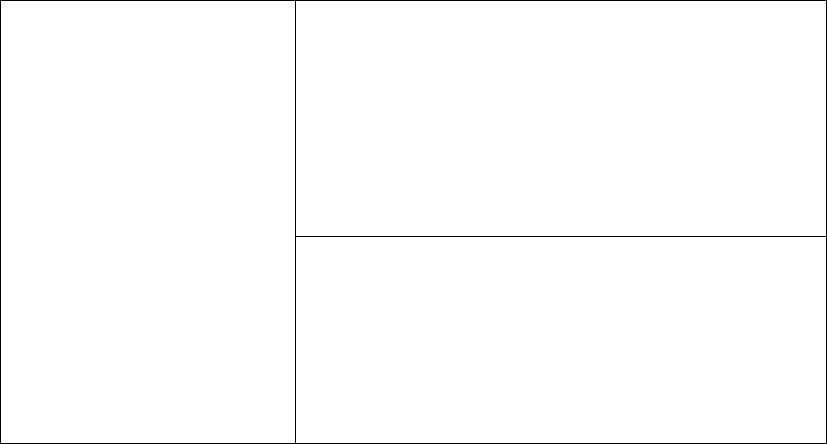
\includegraphics[width=0.6\columnwidth]{figures/partition.pdf}
  \caption{Environment partitioning}
  \label{fig:partition}
\end{figure}

This can be improved by computing the partition according to the position of the coral.

\subsection{Role assignment}

An exploration group can be composed of 1 or 2 agents. If it is a 1-agent group, the only agent plays the role \textsf{explorer}. If it is a 2-agent group, one agent plays the role \textsf{explorer} (the agent farest form the coral), the second one plays the role \textsf{scout}. During these role playings, each agent shares its perceptions with its partner.

\ascomment{}

\subsection{Explorer role playing}

The tasks of the \textsf{explorer} are quite simple:
\begin{enumerate}
\item choose a target position: the near position which is least visited within its partition,
\item compute a path to the target position, using $A^\star$ algorithm,
\item move along the computed path. 
\end{enumerate}

This role playing ends as soon as the \textsf{explorer} perceives a cow.

\ascomment{}

\subsection{Scout role playing}

The role of the \textsf{scout} is to help the \textsf{explorer} to find
cows. As to maximize the number of visited cells, the scout must be positioned
at a distance equal to the double of the perception distance of agents relatively to the
\textsf{explorer}, orthogonally to the direction of the target position from
the viewpoint of the \textsf{explorer} (figure~\ref{fig:position})

\begin{figure}[h]
  \centering
  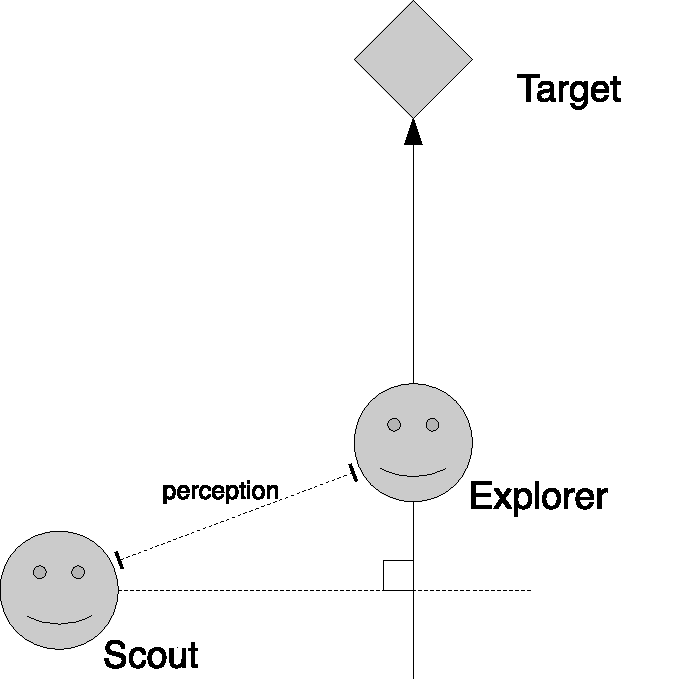
\includegraphics[width=.4\columnwidth]{figures/exploration-positioning.pdf}
  \caption{Position of the \textsf{scout} relatively to the \textsf{explorer} during exploration phase}
  \label{fig:position}
\end{figure}

This requires some coordination with the \textsf{explorer}:
\begin{itemize}
\item the \textsf{explorer} informs the \textsf{scout} of its next target position and its own position (in case the \textsf{scout} does not perceive it),
\item the \textsf{scout} compute its next target position.
\end{itemize}

But before that, the \textsf{scout} must move towards the \textsf{explorer} until it perceives it. 

This role playing ends as soon as the \textsf{explorer} (which is now a \textsf{tracker}) a \textsf{herder}, as to begin the herding phase.

\ascomment{}

\subsection{Tracker role playing}
\label{sec:tracker-role-playing}

Once the \textsf{explorer} perceives a cow, it plays the \textsf{tracker} role which aims at evaluating the size of the cluster of cows. The \textsf{tracker} does the following tasks:
\begin{enumerate}
\item compute the next target position: a position at the opposite of the coral position according the center of the cluster,
\item circle the coral as to reach the target position,
\item count the perceived cows until it reaches the target position (maintaining a counter $\mathrm size$),
\item once the target position is reached, decide whether the group must split, grow or remain as it is, with respect to the following rules:
\begin{itemize}
\item if ($\mathrm{size} \leq \tau < \tau_{\mathrm{max}}$) then split the group: one \textsf{herder} is sufficient to herd the cluster to the coral; the \textsf{scout} plays now the \textsf{explorer} role,
\item if ($\tau < \mathrm{size} \leq \tau_{\mathrm{max}}$) then the group is kept: the two agents are sufficient; the \textsf{explorer} plays now the \textsf{herder} role and the \textsf{scout} now plays the \textsf{herdboy} role,
\item if ($\tau < \tau_{\mathrm{max}} < \mathrm{size}$) then the group must recruit nearest \textsf{explorer} agents or negotiate with other \textsf{herder} agents to recruit \textsf{herdboy} agents.
\end{itemize}
\end{enumerate}

Negotiation between \textsf{herders} will depends on:
\begin{itemize}
\item the sizes of the respective clusters,
\item the distance between the agents to recruit and the recruiting agent.
\end{itemize}

At the end of this role playing, the \textsf{explorer} is positioned so as to have the cluster between itself and the coral. In this position, it only has to move to the coral to ``push'' the cluster in the good direction.

During this phase, the \textsf{scout} continues to play this role.

\ascomment{}

\section{Herding}

This phase starts as soon as a \textsf{tracker} becomes a \textsf{herder}. At the same moment, the \textsf{scout} becomes either a \textsf{herdboy} or an \textsf{explorer}, depending on the size of the cluster.

\subsection{Herder role playing}

The role of a \textsf{herder} is to guide a cluster to the coral. As said before, the cluster (its center) is positioned between the \textsf{herder} and the coral.

Mainly, the tasks for a \textsf{herder} are:
\begin{enumerate}
\item update the size of the cluster\footnote{necessary to detect whether a cluster is too big},
\item recruit if necessary (see section \ref{sec:tracker-role-playing}),
\item compute the center of the cluster,
\item compute the target position with respect of the position of the coral and the center of the cluster,
\item compute the path to reach this position by using $A^\star$,
\item compute its next position according to the previous information,
\item inform its \textsf{herdboys} of this position, 
\item compute the path to the next position using $A^\star$,
\item move to its next position.
\end{enumerate}

\ascomment{}

We can identify some \textbf{exceptions}:
\begin{itemize}
\item \textbf{immobile cluster}: if the cluster does not move for $t_{\mathrm max}$ steps, the \textsf{herder} must change its target direction by adding an $\alpha$ angle to the direction.
\item \textbf{two clusters meet}: if two clusters start to merge, \textsf{herders} must decide whether the cluster must merge or not. This implies negotiation between the two agents depending on the total size of the cluster.
\item \textbf{cluster too big}: if the cluster $\mathrm{size} > \tau_{\mathrm
    supermax} (\tau_{\mathrm supermax} > \tau_{\mathrm max})$, it must split into two clusters. As to do this, the \textsf{herder} go to the center of the cluster as to create a breach in the cluster (and becomes then \textsf{ranger}). New \textsf{herders} must be chosen among the \textsf{herdboys} for the new clusters. The \textsf{ranger} becomes an \textsf{explorer} as to be easily recruited by the new \textsf{herders}.
\end{itemize}

\ascomment{}

\subsection{Herdboy role playing}

The \textsf{herdboy} role is quite simple: it helps the \textsf{herder} to herd a cluster to the coral. \textsf{Herdboys} are led by one \textsf{herder}. Once a \textsf{herder} begins to herd a cluster to the coral, some \textsf{herdboys} may help it to achieve this task.

\textsf{Herdboys}' tasks are:
\begin{enumerate}
\item detect close clusters, as to decide whether they merge or not,
\item compute its next position thanks to information coming from its \textsf{herder}: each \textsf{herdboy} moves to a position near the \textsf{herder} around the cluster. E.g. if the \textsf{herder} is on the line from coral to cluster, the first \textsf{herdboy} position itself on a line at 10� left from the \textsf{herder}'s position, the second one on a line at 10� right, etc.
\item compute the path to the next position using $A^\star$, 
\item move the next position.
\end{enumerate}

If the cluster too big exception occurs, \textsf{herdboys} must try to enter in the breach created by the \textsf{herder} to help the cluster splitting.

\ascomment{}

\subsection{Ranger role playing}

The \textsf{ranger}'s role is to create a breach inside a big cluster to create two separate cluster. Once it is done, it becomes an \textsf{explorer}.
The idea is to split the cluster by letting the cows move by side, since herdboys move to the position of the ranger and do not constrain cows anymore.
Once it is done, the side of the cluster are free, and cows can move by side.
It leads \textsf{herdboys} during this stage.

\textsf{Ranger}'s tasks are:
\begin{enumerate}
\item inform \textsf{herdboys} they have to move to its position around the cluster,
\item compute its next target position: the point at the opposite of its current position according to the center of the cluster,
\item compute the path to this position using $A^\star$,
\item move to the next position. 
\end{enumerate}

\ascomment{}


\section{Some algorithms}

\subsection{Cluster identification}

some how based on Hierarchical Clustering Algorithms
http://home.dei.polimi.it/matteucc/Clustering/tutorial\_html

\begin{verbatim}
V = set of all seen cows sorted by the distance to the center of V
C = { the cow near to the center of V }

add = true
while (add)
 add = false
 for all v in V
   if (some cow in C sees v)
     add v in C
     add = true
\end{verbatim}

\subsection{Merging clusters/groups}

performed by each herder of group gi
\begin{verbatim}
for all herding groups gj with id > gi.id

let Si the set of cows seen by agents of group gi
let Sj the set of cows seen by agents of group gj
if Si intersect Sj not empty
   // merge condition
   group gj is removed from the organisation
   all agents from gj adopt scouter in gi
\end{verbatim}


\section{TODO list}

\begin{enumerate}
\item add \emph{AgentSpeak} specification for each role
\item specify the dynamic role-chart with roles and triggers to sum up the role dynamics
\end{enumerate}

\end{document}
